\pagestyle{myheadings}\markboth{SOLUTIONS}{SOLUTIONS}
\phantomsection\section*{Solutions}\label{sec:sols}
\addcontentsline{toc}{section}{Solutions}

\phantomsection\subsection*{Chapter 1 Solutions}
\addcontentsline{toc}{subsection}{S.1~~~Chapter 1 Solutions}

\begin{solution}{\ref{ex:ch1-maps}}{
    The diagram of \(f \colon \Omega_{6} \to \Omega_{5}\) is Figure~\ref{fig:ch1-maps}.
        \begin{figure}[h]
        \centering
        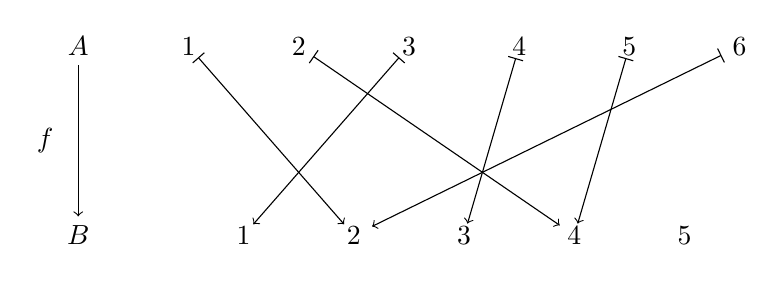
\begin{tikzpicture}[xscale=1.4,yscale=0.6]%  [xscale=1.4,yscale=0.8]
            \foreach \x in {1,2,3,4,5,6} \node at (\x,2) {\(\x\)};\node at (0,2) {\(A\)};
            \foreach \x in {1,2,3,4,5} \node at (\x+0.5,-2) {\(\x\)};\node at (0,-2) {\(B\)};
            \draw[->] (0,1.6) -- (0,-1.6); \node at (-0.3,0) {\(f\)};

            \draw[|->] (1.088,1.766) -- (2.412,-1.766);
            \draw[|->] (2.132,1.788) -- (4.368,-1.788);
            \draw[|->] (2.912,1.766) -- (1.588,-1.766);
            \draw[|->] (3.969,1.752) -- (3.531,-1.752);
            \draw[|->] (4.969,1.752) -- (4.531,-1.752);
            \draw[|->] (5.835,1.812) -- (2.665,-1.812);
        \end{tikzpicture}
        \caption{The diagram of the map \(f \colon \Omega_{6} \to \Omega_{5}\).}
        \label{fig:ch1-maps}
    \end{figure}\vspace*{-10pt}

    This map is not injective as both \(1, 6 \in \Omega_{6}\) map to \(1 \in \Omega_{5}\), for example. This shows that \(f\) is not one-to-one. Similarly, the map is not surjective since no element in \(\Omega_{6}\) maps to \(5 \in \Omega_{5}\). Since \(f\) is not both injective and surjective, it is not bijective.
}\end{solution}

\begin{solution}{\ref{ex:ch1-fourmethods}}{
    Let \(\sigma = (1 \q 6 \q 4 \q 2 \q 5)\) and \(\gamma = (1 \q 5 \q 2 \q 4 \q 6)\). In mapping notation, we write
    \[
    \begin{array}{c}
        \sigma(1) = 6,\quad \sigma(2) = 5,\quad \sigma(3) = 3,\quad \sigma(4) = 2,\quad \sigma(5) = 1,\quad \sigma(6) = 4,\\[8pt]
        \gamma(1) = 5,\quad \gamma(2) = 4,\quad \gamma(3) = 3,\quad \gamma(4) = 6,\quad \gamma(5) = 2,\quad \gamma(6) = 1.
    \end{array}
    \]
    In two line form, these are written
    \[
    \sigma = \begin{pmatrix}
        1 & 2 & 3 & 4 & 5 & 6\\
        6 & 5 & 3 & 2 & 1 & 4\\
    \end{pmatrix},\quad \gamma = \begin{pmatrix}
        1 & 2 & 3 & 4 & 5 & 6\\
        5 & 4 & 3 & 6 & 2 & 1\\
    \end{pmatrix}.
    \]
    In diagrammatic form, we have Figure~\ref{fig:diagrammaticformexercises}.

    \begin{figure}[h]
        \centering
        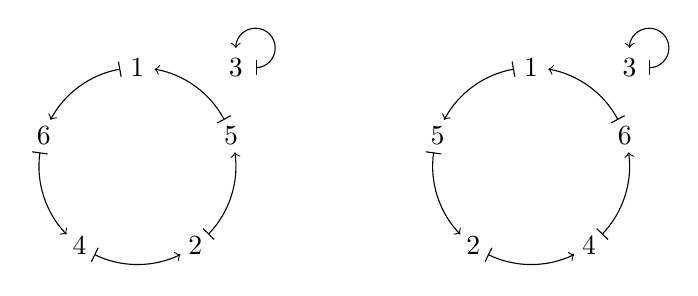
\begin{tikzpicture}[scale=1.25]
            \node at (0,1) {\(1\)};
            \node at (-0.951,0.309) {\(6\)};
            \node at (-0.588,-0.809) {\(4\)};
            \node at (0.588,-0.809) {\(2\)};
            \node at (0.951,0.309) {\(5\)};

            \draw[|->,rotate around={10:(0, 0)}] (0, 1) arc (90:142:1);
            \draw[|->,rotate around={82:(0, 0)}] (0, 1) arc (90:142:1);
            \draw[|->,rotate around={154:(0, 0)}] (0, 1) arc (90:142:1);
            \draw[|->,rotate around={226:(0, 0)}] (0, 1) arc (90:142:1);
            \draw[|->,rotate around={298:(0, 0)}] (0, 1) arc (90:142:1);

            \node at (1,1) {\(3\)};\draw[|->] (1.2,1) arc (-90:180:0.2);

            \begin{scope}[shift={(4,0)}]
                \node at (0,1) {\(1\)};
                \node at (-0.951,0.309) {\(5\)};
                \node at (-0.588,-0.809) {\(2\)};
                \node at (0.588,-0.809) {\(4\)};
                \node at (0.951,0.309) {\(6\)};

                \draw[|->,rotate around={10:(0, 0)}] (0, 1) arc (90:142:1);
                \draw[|->,rotate around={82:(0, 0)}] (0, 1) arc (90:142:1);
                \draw[|->,rotate around={154:(0, 0)}] (0, 1) arc (90:142:1);
                \draw[|->,rotate around={226:(0, 0)}] (0, 1) arc (90:142:1);
                \draw[|->,rotate around={298:(0, 0)}] (0, 1) arc (90:142:1);

                \node at (1,1) {\(3\)};\draw[|->] (1.2,1) arc (-90:180:0.2);
            \end{scope}
        \end{tikzpicture}
        \caption{Diagrammatic form of \(\sigma\) (left) and \(\gamma\) (right).}
        \label{fig:diagrammaticformexercises}
    \end{figure}

    We now find the product \(\sigma\gamma\) using the right-to-left reading convention and then the left-to-right reading convention.

    \textsc{1.~~~Right-to-left}

    \ulsc{Maps notation:} We find the composition \(\sigma\circ\gamma\) by considering each element in \(\Omega_{6}\):
    \[
    \begin{array}{ccc}
        \sigma\big(\gamma(1)\big) = \sigma(5) = 1, \hspace{20pt} & \sigma\big(\gamma(2)\big) = \sigma(4) = 2, \hspace{20pt} & \sigma\big(\gamma(3)\big) = \sigma(3) = 3, \\[8pt]
        \sigma\big(\gamma(4)\big) = \sigma(6) = 4, \hspace{20pt} & \sigma\big(\gamma(5)\big) = \sigma(2) = 5, \hspace{20pt} & \sigma\big(\gamma(6)\big) = \sigma(1) = 6. \\
    \end{array}
    \]
    Thus
    \[
    \sigma\gamma(1) = 1,\quad \sigma\gamma(2) = 2,\quad \sigma\gamma(3) = 3,\quad \sigma\gamma(4) = 4,\quad \sigma\gamma(5) = 5,\quad \sigma\gamma(6) = 6,
    \]
    so \(\sigma\gamma = (1)(2)(3)(4)(5)(6)\).
    % \[
    % \sigma\gamma = (1)(2)(3)(4)(5)(6).
    % \]

    \ulsc{Two-line form:} To find the composition \(\sigma\circ\gamma\) using the two line form, we write
    \[
    \sigma\gamma = \begin{pmatrix}
        1 & 2 & 3 & 4 & 5 & 6\\
        6 & 5 & 3 & 2 & 1 & 4\\
    \end{pmatrix}\begin{pmatrix}
        1 & 2 & 3 & 4 & 5 & 6\\
        5 & 4 & 3 & 6 & 2 & 1\\
    \end{pmatrix}.
    \]
    We read this right-to-left. We will colour the columns accordingly:
    \[
    \sigma\gamma = \begin{pmatrix}
        \textcolor{orange!90!black}{1} & \textcolor{yellow!90!black}{2} & \textcolor{blue!90!black}{3} & \textcolor{purple!90!black}{4} & \textcolor{red!90!black}{5} & \textcolor{green!90!black}{6}\\
        \textcolor{orange!90!black}{6} & \textcolor{yellow!90!black}{5} & \textcolor{blue!90!black}{3} & \textcolor{purple!90!black}{2} & \textcolor{red!90!black}{1} & \textcolor{green!90!black}{4}\\
    \end{pmatrix}\begin{pmatrix}
        \textcolor{red!90!black}{1} & \textcolor{purple!90!black}{2} & \textcolor{blue!90!black}{3} & \textcolor{green!90!black}{4} & \textcolor{yellow!90!black}{5} & \textcolor{orange!90!black}{6}\\
        \textcolor{red!90!black}{5} & \textcolor{purple!90!black}{4} & \textcolor{blue!90!black}{3} & \textcolor{green!90!black}{6} & \textcolor{yellow!90!black}{2} & \textcolor{orange!90!black}{1}\\
    \end{pmatrix}.
    \]
    The colours indicate that
    \[
    \sigma\gamma = \begin{pmatrix}
        1 & 2 & 3 & 4 & 5 & 6\\
        1 & 2 & 3 & 4 & 5 & 6\\
    \end{pmatrix}.
    \]

    \ulsc{Diagrams:} To find the the composition \(\sigma\circ\gamma\) using diagrams, we draw the following:

    \begin{figure}[h]
        \centering
        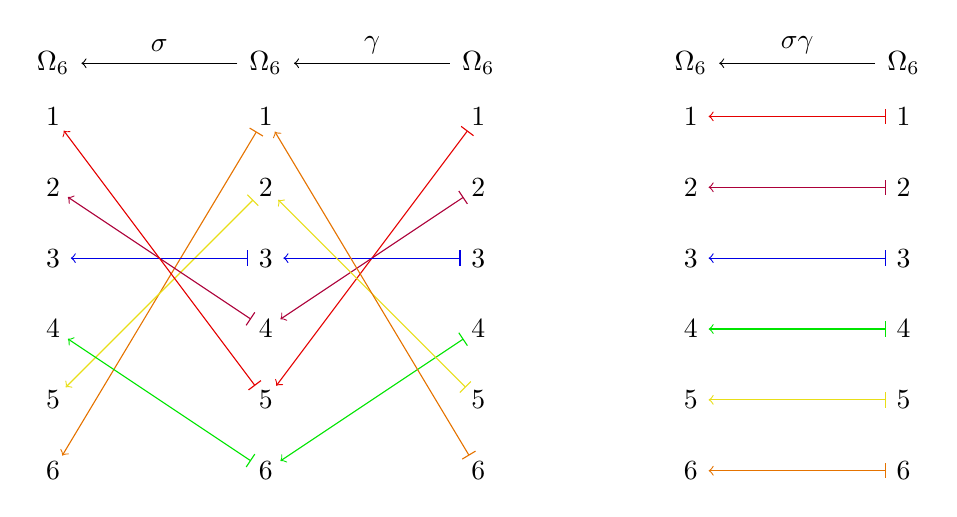
\begin{tikzpicture}[scale=0.9]
            \foreach \x in {1,2,3,4,5,6}
                \node at (-3,-\x) {\(\x\)};
            \foreach \x in {1,2,3,4,5,6}
                \node at (0,-\x) {\(\x\)};
            \foreach \x in {1,2,3,4,5,6}
                \node at (3,-\x) {\(\x\)};
            \foreach \x in {-3,0,3}
                \node at (\x,-0.25) {\(\Omega_{6}\)};
            \node at (-1.5,0) {\(\sigma\)};\node at (1.5,0) {\(\gamma\)};

            \draw[->] (-0.4,-0.25) -- (-2.6,-0.25);
            \draw[->] (2.6,-0.25) -- (0.4,-0.25);

            \draw[|->,red!90!black](2.85,-1.2) -- (0.15,-4.8);
            \draw[|->,purple!90!black](2.792,-2.139) -- (0.208,-3.861);
            \draw[|->,blue!90!black](2.75,-3) -- (0.25,-3);
            \draw[|->,green!90!black](2.792,-4.139) -- (0.208,-5.861);
            \draw[|->,yellow!90!black](2.823,-4.823) -- (0.177,-2.177);
            \draw[|->,orange!90!black](2.871,-5.786) -- (0.129,-1.214);

            \draw[|->,orange!90!black](-0.129,-1.214) -- (-2.871,-5.786);
            \draw[|->,yellow!90!black](-0.177,-2.177) -- (-2.823,-4.823);
            \draw[|->,blue!90!black](-0.25,-3) -- (-2.75,-3);
            \draw[|->,purple!90!black](-0.208,-3.861) -- (-2.792,-2.139);
            \draw[|->,red!90!black](-0.15,-4.8) -- (-2.85,-1.2);
            \draw[|->,green!90!black](-0.208,-5.861) -- (-2.792,-4.139);

            \begin{scope}[shift={(6,0)}]
                \foreach \x in {1,2,3,4,5,6}
                    \node at (0,-\x) {\(\x\)};
                \foreach \x in {1,2,3,4,5,6}
                    \node at (3,-\x) {\(\x\)};
                \foreach \x in {0,3}
                    \node at (\x,-0.25) {\(\Omega_{6}\)};
                \node at (1.5,0) {\(\sigma\gamma\)};\draw[->] (2.6,-0.25) -- (0.4,-0.25);

                \draw[|->,red!90!black](2.75,-1) -- (0.25,-1);
                \draw[|->,purple!90!black](2.75,-2) -- (0.25,-2);
                \draw[|->,blue!90!black](2.75,-3) -- (0.25,-3);
                \draw[|->,green!90!black](2.75,-4) -- (0.25,-4);
                \draw[|->,yellow!90!black](2.75,-5) -- (0.25,-5);
                \draw[|->,orange!90!black](2.75,-6) -- (0.25,-6);
            \end{scope}
        \end{tikzpicture}
        \caption{The diagram of \(\gamma\sigma\) as a composition (left) and its simplification (right).}
        \label{fig:sol_1.2a}
    \end{figure}

    This gives \(\gamma\sigma = (1)(2)(3)(4)(5)(6)\).

    \ulsc{One-line form:} Finally, to find the the composition \(\sigma\circ\gamma\) using one-line form, we write
    \[
    \sigma\circ\gamma = (1 \q 6 \q 4 \q 2 \q 5)(1 \q 5 \q 2 \q 4 \q 6).
    \]
    This is read right-to-left to give
    \[
    1 \xmapsto{\gamma} 5 \xmapsto{\sigma} 1,\quad 2 \xmapsto{\gamma} 4 \xmapsto{\sigma} 2,\quad 3 \xmapsto{\gamma} 3 \xmapsto{\sigma} 3,\quad 4 \xmapsto{\gamma} 6 \xmapsto{\sigma} 4,\quad 5 \xmapsto{\gamma} 2 \xmapsto{\sigma} 5,\quad 6 \xmapsto{\gamma} 1 \xmapsto{\sigma} 6.
    \]
    Hence \(\sigma\gamma = (1)(2)(3)(4)(5)(6)\).

    \textsc{2.~~~Left-to-right}

    \ulsc{Maps notation:} We find the product \(\sigma\cdot\gamma\) by considering each element in \(\Omega_{6}\). Note that the product \(\sigma\cdot\gamma\) evaluates \(\sigma\) first and then \(\gamma\), so
    \[
    \begin{array}{ccc}
        \gamma\big(\sigma(1)\big) = \gamma(6) = 1, \hspace{20pt} & \gamma\big(\sigma(2)\big) = \gamma(5) = 2, \hspace{20pt} & \gamma\big(\sigma(3)\big) = \gamma(3) = 3, \\[8pt]
        \gamma\big(\sigma(4)\big) = \gamma(2) = 4, \hspace{20pt} & \gamma\big(\sigma(5)\big) = \gamma(1) = 5, \hspace{20pt} & \gamma\big(\sigma(6)\big) = \gamma(4) = 6. \\
    \end{array}
    \]
    Thus
    \[
    \sigma\gamma(1) = 1,\quad \sigma\gamma(2) = 2,\quad \sigma\gamma(3) = 3,\quad \sigma\gamma(4) = 4,\quad \sigma\gamma(5) = 5,\quad \sigma\gamma(6) = 6,
    \]
    so \(\sigma\gamma = (1)(2)(3)(4)(5)(6)\).
    % \[
    % \sigma\gamma = (1)(2)(3)(4)(5)(6).
    % \]

    \ulsc{Two-line form:} To find the product \(\sigma\cdot\gamma\) using the two line form, we write
    \[
    \sigma\gamma = \begin{pmatrix}
        1 & 2 & 3 & 4 & 5 & 6\\
        6 & 5 & 3 & 2 & 1 & 4\\
    \end{pmatrix}\begin{pmatrix}
        1 & 2 & 3 & 4 & 5 & 6\\
        5 & 4 & 3 & 6 & 2 & 1\\
    \end{pmatrix}.
    \]
    We read this left-to-right. We will colour the columns accordingly:
    \[
    \sigma\gamma = \begin{pmatrix}
        \textcolor{red!90!black}{1} & \textcolor{purple!90!black}{2} & \textcolor{blue!90!black}{3} & \textcolor{green!90!black}{4} & \textcolor{yellow!90!black}{5} & \textcolor{red!90!black}{6}\\
        \textcolor{red!90!black}{6} & \textcolor{purple!90!black}{5} & \textcolor{blue!90!black}{3} & \textcolor{green!90!black}{2} & \textcolor{yellow!90!black}{1} & \textcolor{red!90!black}{4}\\
    \end{pmatrix}\begin{pmatrix}
        \textcolor{yellow!90!black}{1} & \textcolor{green!90!black}{2} & \textcolor{blue!90!black}{3} & \textcolor{orange!90!black}{4} & \textcolor{purple!90!black}{5} & \textcolor{red!90!black}{6}\\
        \textcolor{yellow!90!black}{5} & \textcolor{green!90!black}{4} & \textcolor{blue!90!black}{3} & \textcolor{orange!90!black}{6} & \textcolor{purple!90!black}{2} & \textcolor{red!90!black}{1}\\
    \end{pmatrix}.
    \]
    The colours indicate that
    \[
    \sigma\gamma = \begin{pmatrix}
        1 & 2 & 3 & 4 & 5 & 6\\
        1 & 2 & 3 & 4 & 5 & 6\\
    \end{pmatrix}.
    \]

    \ulsc{Diagrams:} To find the the composition \(\sigma\circ\gamma\) using diagrams, we draw the following:

    \begin{figure}[h]
        \centering
        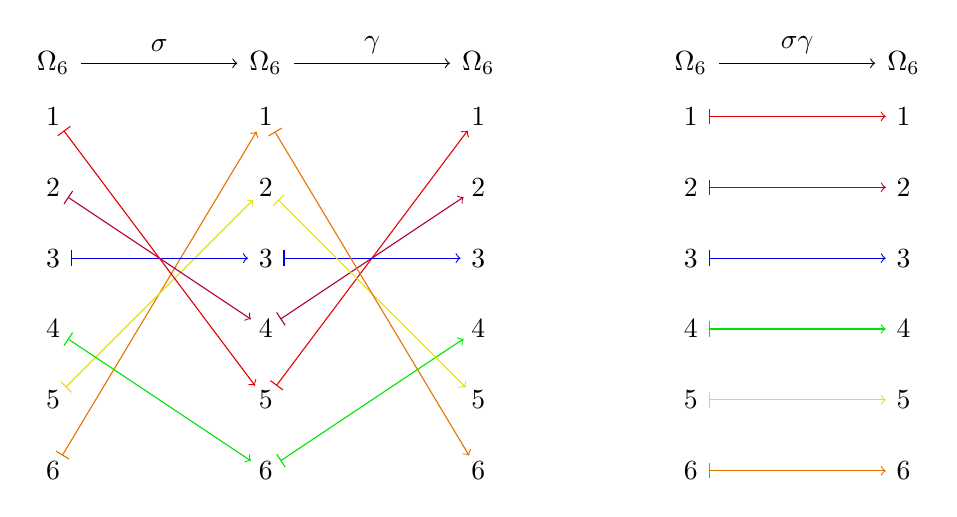
\begin{tikzpicture}[scale=0.9]
            \foreach \x in {1,2,3,4,5,6}
                \node at (-3,-\x) {\(\x\)};
            \foreach \x in {1,2,3,4,5,6}
                \node at (0,-\x) {\(\x\)};
            \foreach \x in {1,2,3,4,5,6}
                \node at (3,-\x) {\(\x\)};
            \foreach \x in {-3,0,3}
                \node at (\x,-0.25) {\(\Omega_{6}\)};
            \node at (-1.5,0) {\(\sigma\)};\node at (1.5,0) {\(\gamma\)};

            \draw[->] (-2.6,-0.25) -- (-0.4,-0.25);
            \draw[->] (0.4,-0.25) -- (2.6,-0.25);

            \draw[<-|,red!90!black](2.85,-1.2) -- (0.15,-4.8);
            \draw[<-|,purple!90!black](2.792,-2.139) -- (0.208,-3.861);
            \draw[<-|,blue!90!black](2.75,-3) -- (0.25,-3);
            \draw[<-|,green!90!black](2.792,-4.139) -- (0.208,-5.861);
            \draw[<-|,yellow!90!black](2.823,-4.823) -- (0.177,-2.177);
            \draw[<-|,orange!90!black](2.871,-5.786) -- (0.129,-1.214);

            \draw[<-|,orange!90!black](-0.129,-1.214) -- (-2.871,-5.786);
            \draw[<-|,yellow!90!black](-0.177,-2.177) -- (-2.823,-4.823);
            \draw[<-|,blue!90!black](-0.25,-3) -- (-2.75,-3);
            \draw[<-|,purple!90!black](-0.208,-3.861) -- (-2.792,-2.139);
            \draw[<-|,red!90!black](-0.15,-4.8) -- (-2.85,-1.2);
            \draw[<-|,green!90!black](-0.208,-5.861) -- (-2.792,-4.139);

            \begin{scope}[shift={(6,0)}]
                \foreach \x in {1,2,3,4,5,6}
                    \node at (0,-\x) {\(\x\)};
                \foreach \x in {1,2,3,4,5,6}
                    \node at (3,-\x) {\(\x\)};
                \foreach \x in {0,3}
                    \node at (\x,-0.25) {\(\Omega_{6}\)};
                \node at (1.5,0) {\(\sigma\gamma\)};\draw[->] (0.4,-0.25) -- (2.6,-0.25);

                \draw[<-|,red!90!black](2.75,-1) -- (0.25,-1);
                \draw[<-|,purple!90!black](2.75,-2) -- (0.25,-2);
                \draw[<-|,blue!90!black](2.75,-3) -- (0.25,-3);
                \draw[<-|,green!90!black](2.75,-4) -- (0.25,-4);
                \draw[<-|,yellow!90!black](2.75,-5) -- (0.25,-5);
                \draw[<-|,orange!90!black](2.75,-6) -- (0.25,-6);
            \end{scope}
        \end{tikzpicture}
        \caption{The diagram of \(\gamma\sigma\) as a product (left) and its simplification (right).}
        \label{fig:sol_1.2b}
    \end{figure}

    This gives \(\gamma\sigma = (1)(2)(3)(4)(5)(6)\).

    \ulsc{One-line form:} Finally, to find the the product \(\sigma\cdot\gamma\) using one-line form, we write
    \[
    \sigma\cdot\gamma = (1 \q 6 \q 4 \q 2 \q 5)(1 \q 5 \q 2 \q 4 \q 6).
    \]
    This is read left-to-right to give
    \[
    1 \xmapsto{\sigma} 5 \xmapsto{\gamma} 1,\quad 2 \xmapsto{\sigma} 4 \xmapsto{\gamma} 2,\quad 3 \xmapsto{\sigma} 3 \xmapsto{\gamma} 3,\quad 4 \xmapsto{\sigma} 6 \xmapsto{\gamma} 4,\quad 5 \xmapsto{\sigma} 2 \xmapsto{\gamma} 5,\quad 6 \xmapsto{\sigma} 1 \xmapsto{\gamma} 6.
    \]
    Hence \(\sigma\gamma = (1)(2)(3)(4)(5)(6)\).
}\end{solution}

\begin{solution}{\ref{ex:ch1-notpermutations}}{
    Let
    \[
    \sigma_{1} = \begin{pmatrix}
        1 & 2 & 3 & 4 & 5 \\
        3 & 2 & 1 & 5 & 4 \\
    \end{pmatrix},\, \sigma_{2} = \begin{pmatrix}
        1 & 2 & 3 & 4 & 5 \\
        5 & 1 & 4 & 2 & 4 \\
    \end{pmatrix},\, \sigma_{3} = \begin{pmatrix}
        1 & 2 & 3 & 4 & 5 \\
        1 & 2 & 3 & 4 & 5 \\
    \end{pmatrix},\, \sigma_{4} = \begin{pmatrix}
        1 & 2 & 3 & 4 & 5 \\
        4 & 1 & 7 & 5 & 3 \\
    \end{pmatrix}.
    \]
    Each of these permutations have five columns, so to be proper permutations each of \(1, 2, 3, 4, 5\) must appear exactly once in the top row and exactly once in the bottom row. This means that the first permutation \(\sigma_{1}\) is a proper permutation, as is the third permutation \(\sigma_{3}\). However, the second permutation \(\sigma_{2}\) has a repeated \(4\) in the bottom row, so it is not a proper permutation. Similarly, the fourth permutation \(\sigma_{4}\) has no \(2\) in the bottom row, and the \(7\) would indicate that the permutation is a map \(\sigma_{4} \colon \Omega_{7} \to \Omega_{7}\). However, the map has not been defined for \(6\) or \(7\) as neither appear on the top row, so \(\sigma_{4}\) is not a well-defined map, and thus not a well-defined permutation either.
}\end{solution}

\begin{solution}{\ref{ex:ch1-frontcover}}{
    The one-line form of the permutation on the front cover is
    \[
    (1 \q 2 \q 3 \q 4 \q 5 \q 6 \q 7 \q 8)
    \]
    and the two-line form is
    \[
    \begin{pmatrix}
        1 & 2 & 3 & 4 & 5 & 6 & 7 & 8\\
        2 & 3 & 4 & 5 & 6 & 7 & 8 & 1\\
    \end{pmatrix}.
    \]
}\end{solution}

\begin{solution}{\ref{ex:ch1-powers}}{
    Let \(\sigma = (1 \q 6 \q 4 \q 2 \q 5)\) and \(\gamma = (1 \q 5 \q 2 \q 4 \q 6)\) be permutations on \(\Omega_{6}\). It is required to compute \(\sigma^{i}\) and \(\gamma^{i}\) for \(i \in \{2, 3, 4, 5, 6\}\). Consider computing \(\sigma^{2}\) with the right-to-left reading convention and then the left-to-right reading convention. In either case, we apply \(\sigma\) first and then \(\sigma\), so that the result is the same in either case. Thus when computing powers of a permutation, one may use either convention.

    We start with the powers of \(\sigma\). We will use the cycle notation method, and leave it to the reader to use the other methods. The square of \(\sigma\) is calculated to be
    \[
    \sigma^{2} = (1 \q 6 \q 4 \q 2 \q 5)(1 \q 6 \q 4 \q 2 \q 5) = (1 \q 4 \q 5 \q 6 \q 2).
    \]
    We see this because
    \[
    1 \xmapsto{\sigma} 6 \xmapsto{\sigma} 4, \hspace{20pt} 2 \xmapsto{\sigma} 5 \xmapsto{\sigma} 1, \hspace{20pt} 3 \xmapsto{\sigma} 3 \xmapsto{\sigma} 3, \hspace{20pt} 4 \xmapsto{\sigma} 2 \xmapsto{\sigma} 5, \hspace{20pt} 5 \xmapsto{\sigma} 1 \xmapsto{\sigma} 6, \hspace{20pt} 6 \xmapsto{\sigma} 4 \xmapsto{\sigma} 2.
    \]
    When one calculates the third power, there are three ways to calculate \(\sigma^{3}\). One can either compute the product \(\sigma\sigma^{2}\) or \(\sigma^{2}\sigma\) since \(\sigma^{2}\) is known, or one can compute \(\sigma^{3}\) directly as \(\sigma\sigma\sigma\). In the first case, using the left-to-right reading convention we compute
    \[
    \sigma\sigma^{2} = (1 \q 6 \q 4 \q 2 \q 5)(1 \q 4 \q 5 \q 6 \q 2).
    \]
    In mapping notation, we see that
    \[
    1 \xmapsto{\sigma} 6 \xmapsto{\sigma^{2}} 2, \hspace{20pt} 2 \xmapsto{\sigma} 5 \xmapsto{\sigma^{2}} 6, \hspace{20pt} 3 \xmapsto{\sigma} 3 \xmapsto{\sigma^{2}} 3, \hspace{20pt} 4 \xmapsto{\sigma} 5 \xmapsto{\sigma^{2}} 1, \hspace{20pt} 5 \xmapsto{\sigma} 1 \xmapsto{\sigma^{2}} 4, \hspace{20pt} 6 \xmapsto{\sigma} 4 \xmapsto{\sigma^{2}} 5,
    \]
    so that
    \[
    \sigma\sigma^{2} = (1 \q 2 \q 6 \q 5 \q 4).
    \]
    This is the same as \(\sigma^{2}\sigma\) using the right-to-left reading convention. Similarly, using the left-to-right reading convention we compute
    \[
    \sigma^{2}\sigma = (1 \q 4 \q 5 \q 6 \q 2)(1 \q 6 \q 4 \q 2 \q 5).
    \]
    In mapping notation, we see that
    \[
    1 \xmapsto{\sigma^{2}} 4 \xmapsto{\sigma} 2, \hspace{20pt} 2 \xmapsto{\sigma^{2}} 1 \xmapsto{\sigma} 6, \hspace{20pt} 3 \xmapsto{\sigma^{2}} 3 \xmapsto{\sigma} 3, \hspace{20pt} 4 \xmapsto{\sigma^{2}} 5 \xmapsto{\sigma} 1, \hspace{20pt} 5 \xmapsto{\sigma^{2}} 6 \xmapsto{\sigma} 4, \hspace{20pt} 6 \xmapsto{\sigma^{2}} 2 \xmapsto{\sigma} 5,
    \]
    so that
    \[
    \sigma^{2}\sigma = (1 \q 2 \q 6 \q 5 \q 4).
    \]
    This is the same as \(\sigma\sigma^{2}\) using the right-to-left reading convention. In the final case, we compute
    \[
    \sigma\sigma\sigma = (1 \q 6 \q 4 \q 2 \q 5)(1 \q 6 \q 4 \q 2 \q 5)(1 \q 6 \q 4 \q 2 \q 5).
    \]
    In mapping notation, we see that
    \[
    \begin{array}{c}
        1 \xmapsto{\sigma} 6 \xmapsto{\sigma} 4 \xmapsto{\sigma} 2, \hspace{20pt} 2 \xmapsto{\sigma} 5 \xmapsto{\sigma} 1 \xmapsto{\sigma} 6, \hspace{20pt} 3 \xmapsto{\sigma} 3 \xmapsto{\sigma} 3 \xmapsto{\sigma} 3,\\
        4 \xmapsto{\sigma} 2 \xmapsto{\sigma} 5 \xmapsto{\sigma} 1, \hspace{20pt} 5 \xmapsto{\sigma} 1 \xmapsto{\sigma} 6 \xmapsto{\sigma} 4, \hspace{20pt} 6 \xmapsto{\sigma} 4 \xmapsto{\sigma} 2 \xmapsto{\sigma} 5.
    \end{array}
    \]
    Thus we have
    \[
    \sigma\sigma\sigma = (1 \q 2 \q 6 \q 5 \q 4).
    \]
    In each case, we find that
    \[
    \sigma^{3} = (1 \q 2 \q 6 \q 5 \q 4).
    \]
    When finding powers of permutations, any one of the three methods can be used. We now find the remaining powers of \(\sigma\).
    \[
    \begin{array}{c}\hline\\[-15pt]\hline\\[-12pt]
        \quad\sigma^{4} = \sigma\sigma^{3} = (1 \q 6 \q 4 \q 2 \q 5)(1 \q 2 \q 6 \q 5 \q 4) = (1 \q 5 \q 2 \q 4 \q 6)\quad \\[2pt]
        \quad\sigma^{5} = \sigma\sigma^{4} = (1 \q 6 \q 4 \q 2 \q 5)(1 \q 5 \q 2 \q 4 \q 6) = (1)(2)(3)(4)(5)(6)\quad \\[2pt]
        \quad\sigma^{6} = \sigma\sigma^{5} = (1 \q 6 \q 4 \q 2 \q 5)(1)(2)(3)(4)(5)(6) = (1 \q 6 \q 4 \q 2 \q 5) = \sigma\quad \\[2pt]\hline\\[-15pt]\hline
    \end{array}
    \]
    The fifth power \(\sigma^{5}\) is an example of the \textit{identity permutation} which maps every element to itself. In Section~\(*\) we put this identity permutation in a formal setting. We also note that the sixth power \(\sigma^{6}\) is equal to \(\sigma\) itself, and that the powers of permutations always cycle back to themselves. This will also be put into a formal setting in Section~\ref{sec:theorems}.

    We now find the powers of \(\gamma = (1 \q 5 \q 2 \q 4 \q 6)\).
    \[
    \begin{array}{c}\hline\\[-15pt]\hline\\[-12pt]
        \quad\gamma^{2} = \gamma\gamma = (1 \q 5 \q 2 \q 4 \q 6)(1 \q 5 \q 2 \q 4 \q 6) = (1 \q 2 \q 6 \q 5 \q 4)\quad \\[2pt]
        \quad\gamma^{3} = \gamma\gamma^{2} = (1 \q 5 \q 2 \q 4 \q 6)(1 \q 2 \q 6 \q 5 \q 4) = (1 \q 4 \q 5 \q 6 \q 2)\quad \\[2pt]
        \quad\gamma^{4} = \gamma\gamma^{3} = (1 \q 5 \q 2 \q 4 \q 6)(1 \q 4 \q 5 \q 6 \q 2) = (1 \q 6 \q 4 \q 2 \q 5)\quad \\[2pt]
        \quad\gamma^{5} = \gamma\gamma^{4} = (1 \q 5 \q 2 \q 4 \q 6)(1 \q 6 \q 4 \q 2 \q 5) = (1)(2)(3)(4)(5)(6)\quad \\[2pt]
        \quad\gamma^{6} = \gamma\gamma^{5} = (1 \q 5 \q 2 \q 4 \q 6)(1)(2)(3)(4)(5)(6) = (1 \q 5 \q 2 \q 4 \q 6) = \gamma\quad \\[2pt]
        \hline\\[-15pt]\hline
    \end{array}
    \]
    Finally, we compare the powers of \(\sigma\) and \(\gamma\). We see that
    \[
    \sigma = \gamma^{4}, \hspace{20pt} \sigma^{2} = \gamma^{3}, \hspace{20pt} \sigma^{3} = \gamma^{2}, \hspace{20pt} \sigma^{4} = \gamma.
    \]
    From these we can determine that \(\sigma\gamma = (1)(2)(3)(4)(5)(6)\), which means that \(\gamma\) is the \textit{inverse} of \(\sigma\). Again, this is put in a formal setting in Section~\ref{sec:theorems}.
}\end{solution}

\begin{solution}{\ref{ex:ch1-rtl&ltr}}{\begin{itemize}[nolistsep]
        \item[(a)] \q$(2 \q 4 \q 6 \q 1 \q 3 \q 5)(2 \q 1)(4 \q 3)(6 \q 5)(2 \q 6 \q 3)(4 \q 1 \q 5)$;
        \item[(b)] \q$(1 \q 2 \q 3)(2 \q 3 \q 4)(3 \q 4 \q 5)(3 \q 2 \q 1)(4 \q 3 \q 2)(5 \q 4 \q 3)$;
        \item[(c)] \q$(1 \q 2 \q 3 \q 4)(3 \q 6 \q 5 \q 2 \q 1 \q 4)(1 \q 4 \q 3 \q 2)$;
        \item[(d)] \q$(1 \q 2)(1 \q 3)(1 \q 4)(1 \q 5)(1 \q 6)(1 \q 7)(1 \q 8)$;
    \end{itemize}
    We start with the right-to-left reading convention. We will use the maps notation to determine the products. Each of the arrows in part (a) of this exercise correspond to the permutations from right to left.

    (a) The product is
    \[
    (2 \q 4 \q 6 \q 1 \q 3 \q 5)(2 \q 1)(4 \q 3)(6 \q 5)(2 \q 6 \q 3)(4 \q 1 \q 5).
    \]
    There are six cycles on six elements, and we will use them without labels for this solution.
    \[
    \begin{array}{c}
        1 \mapsto 5 \mapsto 5 \mapsto 6 \mapsto 6 \mapsto 6 \mapsto 1, \hspace{20pt} 2 \mapsto 2 \mapsto 6 \mapsto 5 \mapsto 5 \mapsto 5 \mapsto 2,\\
        3 \mapsto 3 \mapsto 2 \mapsto 2 \mapsto 2 \mapsto 1 \mapsto 3, \hspace{20pt} 4 \mapsto 1 \mapsto 1 \mapsto 1 \mapsto 1 \mapsto 2 \mapsto 4,\\
        5 \mapsto 4 \mapsto 4 \mapsto 4 \mapsto 3 \mapsto 3 \mapsto 5, \hspace{20pt} 6 \mapsto 6 \mapsto 3 \mapsto 3 \mapsto 4 \mapsto 4 \mapsto 6.
    \end{array}
    \]
    Thus we see that
    \[
    (2 \q 4 \q 6 \q 1 \q 3 \q 5)(2 \q 1)(4 \q 3)(6 \q 5)(2 \q 6 \q 3)(4 \q 1 \q 5) = (1)(2)(3)(4)(5)(6).
    \]

    (b) The product is
    \[
    (1 \q 2 \q 3)(2 \q 3 \q 4)(3 \q 4 \q 5)(3 \q 2 \q 1)(4 \q 3 \q 2)(5 \q 4 \q 3).
    \]
    Again, there are six cycles that we use without labels but with five elements.
    \[
    \begin{array}{c}
        1 \mapsto 1 \mapsto 1 \mapsto 3 \mapsto 4 \mapsto 2 \mapsto 3, \hspace{20pt} 2 \mapsto 2 \mapsto 4 \mapsto 4 \mapsto 5 \mapsto 5 \mapsto 5,\\
        3 \mapsto 5 \mapsto 5 \mapsto 5 \mapsto 3 \mapsto 4 \mapsto 4, \hspace{20pt} 4 \mapsto 3 \mapsto 2 \mapsto 1 \mapsto 1 \mapsto 1 \mapsto 2,\\
        5 \mapsto 4 \mapsto 3 \mapsto 2 \mapsto 2 \mapsto 3 \mapsto 1.
    \end{array}
    \]
    Thus we see that
    \[
    (1 \q 2 \q 3)(2 \q 3 \q 4)(3 \q 4 \q 5)(3 \q 2 \q 1)(4 \q 3 \q 2)(5 \q 4 \q 3) = (1 \q 3 \q 4 \q 2 \q 5).
    \]

    (c) The product is
    \[
    (1 \q 2 \q 3 \q 4)(3 \q 6 \q 5 \q 2 \q 1 \q 4)(1 \q 4 \q 3 \q 2).
    \]
    There are three cycles on six elements.
    \[
    \begin{array}{c}
        1 \mapsto 4 \mapsto 3 \mapsto 4, \hspace{20pt} 2 \mapsto 1 \mapsto 4 \mapsto 1, \hspace{20pt} 3 \mapsto 2 \mapsto 1 \mapsto 2,\\
        4 \mapsto 3 \mapsto 6 \mapsto 6, \hspace{20pt} 5 \mapsto 5 \mapsto 2 \mapsto 3, \hspace{20pt} 6 \mapsto 6 \mapsto 5 \mapsto 5.
    \end{array}
    \]
    Thus we see that
    \[
    (1 \q 2 \q 3 \q 4)(3 \q 6 \q 5 \q 2 \q 1 \q 4)(1 \q 4 \q 3 \q 2) = (1 \q 4 \q 6 \q 5 \q 3 \q 2).
    \]

    (d) The product is
    \[
    (1 \q 2)(1 \q 3)(1 \q 4)(1 \q 5)(1 \q 6)(1 \q 7)(1 \q 8).
    \]
    There are seven cycles on eight elements.
    \[
    \begin{array}{cc}
        1 \mapsto 8 \mapsto 8 \mapsto 8 \mapsto 8 \mapsto 8 \mapsto 8 \mapsto 8,&\hspace{20pt}
        2 \mapsto 2 \mapsto 2 \mapsto 2 \mapsto 2 \mapsto 2 \mapsto 2 \mapsto 1,\\
        3 \mapsto 3 \mapsto 3 \mapsto 3 \mapsto 3 \mapsto 3 \mapsto 1 \mapsto 2,&\hspace{20pt}
        4 \mapsto 4 \mapsto 4 \mapsto 4 \mapsto 4 \mapsto 1 \mapsto 3 \mapsto 3,\\
        5 \mapsto 5 \mapsto 5 \mapsto 5 \mapsto 1 \mapsto 4 \mapsto 4 \mapsto 4,&\hspace{20pt}
        6 \mapsto 6 \mapsto 6 \mapsto 1 \mapsto 5 \mapsto 5 \mapsto 5 \mapsto 5,\\
        7 \mapsto 7 \mapsto 1 \mapsto 6 \mapsto 6 \mapsto 6 \mapsto 6 \mapsto 6,&\hspace{20pt}
        8 \mapsto 1 \mapsto 7 \mapsto 7 \mapsto 7 \mapsto 7 \mapsto 7 \mapsto 7.
    \end{array}
    \]
    Thus we see that
    \[
    (1 \q 2)(1 \q 3)(1 \q 4)(1 \q 5)(1 \q 6)(1 \q 7)(1 \q 8) = (1 \q 8 \q 7 \q 6 \q 5 \q 4 \q 3 \q 2).
    \]

    We now compute the products with the left-to-right reading convention. Each of the arrows in part (b) of this exercise correspond to the permutations from left to right.

    (a) The product is
    \[
    (2 \q 4 \q 6 \q 1 \q 3 \q 5)(2 \q 1)(4 \q 3)(6 \q 5)(2 \q 6 \q 3)(4 \q 1 \q 5).
    \]
    There are six cycles on six elements.
    \[
    \begin{array}{c}
        1 \mapsto 3 \mapsto 3 \mapsto 4 \mapsto 4 \mapsto 4 \mapsto 1, \hspace{20pt}
        2 \mapsto 4 \mapsto 4 \mapsto 3 \mapsto 3 \mapsto 2 \mapsto 2,\\
        3 \mapsto 5 \mapsto 5 \mapsto 5 \mapsto 6 \mapsto 3 \mapsto 3, \hspace{20pt}
        4 \mapsto 6 \mapsto 6 \mapsto 6 \mapsto 5 \mapsto 5 \mapsto 4,\\
        5 \mapsto 2 \mapsto 1 \mapsto 1 \mapsto 1 \mapsto 1 \mapsto 5,\hspace{20pt}
        6 \mapsto 1 \mapsto 2 \mapsto 2 \mapsto 2 \mapsto 6 \mapsto 6.
    \end{array}
    \]
    Thus we see that
    \[
    (2 \q 4 \q 6 \q 1 \q 3 \q 5)(2 \q 1)(4 \q 3)(6 \q 5)(2 \q 6 \q 3)(4 \q 1 \q 5) = (1)(2)(3)(4)(5)(6).
    \]

    (b) The product is
    \[
    (1 \q 2 \q 3)(2 \q 3 \q 4)(3 \q 4 \q 5)(3 \q 2 \q 1)(4 \q 3 \q 2)(5 \q 4 \q 3).
    \]
    There are six elements on five elements.
    \[
    \begin{array}{c}
        1 \mapsto 2 \mapsto 3 \mapsto 4 \mapsto 4 \mapsto 3 \mapsto 5, \hspace{20pt}
        2 \mapsto 3 \mapsto 4 \mapsto 5 \mapsto 5 \mapsto 5 \mapsto 4,\\
        3 \mapsto 1 \mapsto 1 \mapsto 1 \mapsto 3 \mapsto 2 \mapsto 2, \hspace{20pt}
        4 \mapsto 4 \mapsto 2 \mapsto 2 \mapsto 1 \mapsto 1 \mapsto 1,\\
        5 \mapsto 5 \mapsto 5 \mapsto 3 \mapsto 2 \mapsto 4 \mapsto 3.
    \end{array}
    \]
    Thus we see that
    \[
    (1 \q 2 \q 3)(2 \q 3 \q 4)(3 \q 4 \q 5)(3 \q 2 \q 1)(4 \q 3 \q 2)(5 \q 4 \q 3) = (1 \q 5 \q 3 \q 2 \q 4).
    \]

    (c) The product is
    \[
    (1 \q 2 \q 3 \q 4)(3 \q 6 \q 5 \q 2 \q 1 \q 4)(1 \q 4 \q 3 \q 2).
    \]
    There are three cycles on six elements.
    \[
    \begin{array}{c}
        1 \mapsto 2 \mapsto 1 \mapsto 4, \hspace{20pt} 2 \mapsto 3 \mapsto 6 \mapsto 6, \hspace{20pt} 3 \mapsto 4 \mapsto 3 \mapsto 2,\\
        4 \mapsto 1 \mapsto 4 \mapsto 3, \hspace{20pt} 5 \mapsto 5 \mapsto 2 \mapsto 1, \hspace{20pt} 6 \mapsto 6 \mapsto 5 \mapsto 5.
    \end{array}
    \]
    Thus we see that
    \[
    (1 \q 2 \q 3 \q 4)(3 \q 6 \q 5 \q 2 \q 1 \q 4)(1 \q 4 \q 3 \q 2) = (1 \q 4 \q 3 \q 2 \q 6 \q 5).
    \]

    (d) The product is
    \[
    (1 \q 2)(1 \q 3)(1 \q 4)(1 \q 5)(1 \q 6)(1 \q 7)(1 \q 8).
    \]
    There are seven cycles on eight elements.
    \[
    \begin{array}{c}
        1 \mapsto 2 \mapsto 2 \mapsto 2 \mapsto 2 \mapsto 2 \mapsto 2 \mapsto 2, \hspace{20pt}
        2 \mapsto 1 \mapsto 3 \mapsto 3 \mapsto 3 \mapsto 3 \mapsto 3 \mapsto 3,\\
        3 \mapsto 3 \mapsto 1 \mapsto 4 \mapsto 4 \mapsto 4 \mapsto 4 \mapsto 4, \hspace{20pt}
        4 \mapsto 4 \mapsto 4 \mapsto 1 \mapsto 5 \mapsto 5 \mapsto 5 \mapsto 5,\\
        5 \mapsto 5 \mapsto 5 \mapsto 5 \mapsto 1 \mapsto 6 \mapsto 6 \mapsto 6, \hspace{20pt}
        6 \mapsto 6 \mapsto 6 \mapsto 6 \mapsto 6 \mapsto 1 \mapsto 7 \mapsto 7,\\
        7 \mapsto 7 \mapsto 7 \mapsto 7 \mapsto 7 \mapsto 7 \mapsto 1 \mapsto 8, \hspace{20pt}
        8 \mapsto 8 \mapsto 8 \mapsto 8 \mapsto 8 \mapsto 8 \mapsto 8 \mapsto 1.
    \end{array}
    \]
    Thus we see that
    \[
    (1 \q 2)(1 \q 3)(1 \q 4)(1 \q 5)(1 \q 6)(1 \q 7)(1 \q 8) = (1 \q 2 \q 3 \q 4 \q 5 \q 6 \q 7 \q 8).
    \]

    In (b), (c), and (d), we again see that the reading convention makes a significant difference.
}\end{solution}

\begin{solution}{\ref{ex:ch1-ltronly}}{
    Let \(\sigma = (1 \q 3 \q 2 \q 4)\), \(\gamma = (2 \q 3 \q 4)\), and \(\tau = (1 \q 4 \q 5)\). Recall that, for this exercise only, multiplying on the left and multiplying on the right both use the left-to-right reading convention. We compute each of
    \[
    m_{\sigma}(\gamma),\q m_{\sigma}(\tau),\q m_{\sigma}(\gamma\cdot\tau),\q m_{\sigma}(\tau\cdot\gamma),\q m_{\sigma}(\gamma^{2}),\q m_{\sigma}(\tau^{2})
    \]
    given that (a) \(m\) multiplies on the left, and (b) \(m\) multiplies on the right. We first compute \(\gamma\cdot\tau\) and \(\tau\cdot\gamma\). The first product is
    \[
    \gamma\cdot\tau = (2 \q 3 \q 4)(1 \q 4 \q 5) = (1 \q 4 \q 2 \q 3 \q 5),
    \]
    and the second product is
    \[
    \tau\cdot\gamma = (1 \q 4 \q 5)(2 \q 3 \q 4) = (1 \q 2 \q 3 \q 4 \q 5).
    \]
    We also compute the powers \(\gamma^{2}\) and \(\tau^{2}\). The first power is
    \[
    \gamma^{2} = \gamma\gamma = (2 \q 3 \q 4)(2 \q 3 \q 4) = (2 \q 4 \q 3),
    \]
    and the second power is
    \[
    \tau^{2} = \tau\tau = (1 \q 4 \q 5)(1 \q 4 \q 5) = (1 \q 5 \q 4).
    \]

    (a) Suppose that \(m\) multiplies on the left. Then
    \[
    \begin{array}{rccclclcl}
        m_{\sigma}(\gamma)          & = & \sigma\gamma     & = & (1 \q 3 \q 2 \q 4)(2 \q 3 \q 4)           & = & (1 \q 4)(2)(3)        & = & (1 \q 4),\\
        m_{\sigma}(\tau)            & = & \sigma\tau       & = & (1 \q 3 \q 2 \q 4)(1 \q 4 \q 5)           & = & (1 \q 3 \q 2 \q 5)(4) & = & (1 \q 3 \q 2 \q 5),\\
        m_{\sigma}(\gamma\cdot\tau) & = & \sigma\gamma\tau & = & (1 \q 3 \q 2 \q 4)(1 \q 4 \q 2 \q 3 \q 5) & = & (1 \q 5)(2)(3)(4)     & = & (1 \q 5),\\
        m_{\sigma}(\tau\cdot\gamma) & = & \sigma\tau\gamma & = & (1 \q 3 \q 2 \q 4)(1 \q 2 \q 3 \q 4 \q 5) & = & (1 \q 4 \q 2 \q 5)(3) & = & (1 \q 4 \q 2 \q 5),\\
        m_{\sigma}(\gamma^{2})      & = & \sigma\gamma^{2} & = & (1 \q 3 \q 2 \q 4)(2 \q 4 \q 3)           & = & (1 \q 2 \q 3 \q 4),&&\\
        m_{\sigma}(\tau^{2})        & = & \sigma\tau^{2}   & = & (1 \q 3 \q 2 \q 4)(1 \q 5 \q 4)           & = & (1 \q 3 \q 2)(4 \q 5).&&
    \end{array}
    \]

    (b) Suppose that \(m\) multiplies on the right. Then
    \[
    \begin{array}{rccclclcl}
        m_{\sigma}(\gamma)          & = & \gamma\sigma     & = & (2 \q 3 \q 4)(1 \q 3 \q 2 \q 4)           & = & (1 \q 3)(2)(3)        & = & (1 \q 3),\\
        m_{\sigma}(\tau)            & = & \tau\sigma       & = & (1 \q 4 \q 5)(1 \q 3 \q 2 \q 4)           & = & (1)(2 \q 4 \q 5 \q 3) & = & (2 \q 4 \q 5 \q 3),\\
        m_{\sigma}(\gamma\cdot\tau) & = & \gamma\tau\sigma & = & (1 \q 4 \q 2 \q 3 \q 5)(1 \q 3 \q 2 \q 4) & = & (1)(2)(3 \q 5)(4)     & = & (3 \q 5),\\
        m_{\sigma}(\tau\cdot\gamma) & = & \tau\gamma\sigma & = & (1 \q 2 \q 3 \q 4 \q 5)(1 \q 3 \q 2 \q 4) & = & (1 \q 4 \q 5 \q 3)(2) & = & (1 \q 4 \q 5 \q 3),\\
        m_{\sigma}(\gamma^{2})      & = & \gamma^{2}\sigma & = & (2 \q 4 \q 3)(1 \q 3 \q 2 \q 4)           & = & (1 \q 3 \q 4 \q 2),&&\\
        m_{\sigma}(\tau^{2})        & = & \tau^{2}\sigma   & = & (1 \q 5 \q 4)(1 \q 3 \q 2 \q 4)           & = & (1 \q 5)(2 \q 4 \q 3).&&
    \end{array}
    \]
}\end{solution}

\begin{solution}{\ref{ex:ch1-omegainfty}}{
    Let \(\sigma = (2 \q 4 \q 6)\) be a permutation in one-line form. In mapping notation, we have
    \[
    2 \mapsto 4, \hspace{20pt} 4 \mapsto 6, \hspace{20pt} 6 \mapsto 2
    \]
    with every other element mapping to itself. Thus \(\sigma\) is defined on each of
    \[
    \Omega_{6},\q \Omega_{10},\q \Omega_{10^{100}},\q \Omega_{\infty} = \N
    \]
    but also on \(\Omega_{1}\). More formally, the \textit{restriction of \(\sigma\)} to \(\Omega_{1}\) is a proper permutation on \(\Omega_{1}\), written \(\sigma|_{\Omega_{1}}\), and is defined as the same as \(\sigma\) but only on the elements in \(\Omega_{1}\). Since \(\Omega_{1} = \{1\}\) and \(1 \xmapsto{\sigma} 1\), we have that \(1 \xmapsto{\sigma|_{\Omega_{1}}} 1\) and that \(\sigma|_{\Omega_{1}}\colon \Omega_{1} \to \Omega_{1}\) is a well defined permutation. On the other hand, since \(\Omega_{4} = \{1, 2, 3, 4\}\) and \(4 \xmapsto{\sigma} 6\), the restriction of \(\sigma\) to \(\Omega_{4}\), written \(\sigma|_{\Omega_{4}}\), is not a proper permutation on \(\Omega_{4}\) because it maps the element \(4 \in \Omega_{4}\) to the element \(6\) which is not an element of \(\Omega_{4}\). Note that this is not important to know for the rest of the book, but has been included for general interest.

    As a remark, we can regard \textit{every} permutation as a map on \(\Omega_{\infty} = \N\). That is, if \(\sigma\colon \Omega_{n} \to \Omega_{n}\) then \(\sigma\) is a map \(\sigma\colon \Omega_{\infty} \to \Omega_{\infty}\) defined by
    \[
    \begin{cases}
        i \mapsto \sigma(i), & \text{if \(i \in \Omega_{n}\),}\\
        i \mapsto i,         & \text{if \(i \in \Omega_{\infty}\backslash\Omega_{n}\).}
    \end{cases}
    \]
}\end{solution}

\begin{solution}{\ref{ex:ch1-reduced_two-line_form}}{(a) Let
    \[
    \sigma_{1} = (1 \q 3 \q 2 \q 4), \qquad \sigma_{2} = (4 \q 2 \q 1 \q 3), \qquad \sigma_{3} = (2 \q 1 \q 3 \q 4).
    \]
    First suppose that we are using the right-to-left reading convention. We are required to compute the composition \(\sigma_{1}\circ\sigma_{2}\circ\sigma_{3}\). Reading right-to-left and by considering each element in \(\Omega_{4}\), we have
    \[
    1 \xmapsto{\sigma_{3}} 2 \xmapsto{\sigma_{2}} 2 \xmapsto{\sigma_{1}} 3,\qquad
    2 \xmapsto{\sigma_{3}} 1 \xmapsto{\sigma_{2}} 4 \xmapsto{\sigma_{1}} 4,\qquad
    3 \xmapsto{\sigma_{3}} 3 \xmapsto{\sigma_{2}} 1 \xmapsto{\sigma_{1}} 1,\qquad
    4 \xmapsto{\sigma_{3}} 4 \xmapsto{\sigma_{2}} 3 \xmapsto{\sigma_{1}} 2.
    \]
    From this we see that
    \[
    \sigma_{1}\circ\sigma_{2}\circ\sigma_{3} = (3 \q 4 \q 1 \q 2).
    \]
    Now suppose that we are using the left-to-right reading convention. We are required to compute the product \(\sigma_{1}\cdot\sigma_{2}\cdot\sigma_{3}\). Reading left-to-right and by considering each element in \(\Omega_{4}\), we have
    \[
    1 \xmapsto{\sigma_{1}} 1 \xmapsto{\sigma_{2}} 4 \xmapsto{\sigma_{3}} 4,\qquad
    2 \xmapsto{\sigma_{1}} 3 \xmapsto{\sigma_{2}} 1 \xmapsto{\sigma_{3}} 2,\qquad
    3 \xmapsto{\sigma_{1}} 2 \xmapsto{\sigma_{2}} 2 \xmapsto{\sigma_{3}} 1,\qquad
    4 \xmapsto{\sigma_{1}} 4 \xmapsto{\sigma_{2}} 3 \xmapsto{\sigma_{3}} 3.
    \]
    From this we see that
    \[
    \sigma_{1}\cdot\sigma_{2}\cdot\sigma_{3} = (4 \q 2 \q 1 \q 3).
    \]

    (b) Let
    \[
    \gamma_{1} = (2 \q 3 \q 4 \q 1), \qquad \gamma_{2} = (3 \q 4 \q 1 \q 2), \qquad \gamma_{3} = (4 \q 1 \q 2 \q 3).
    \]
    We are required to compute the composition \(\gamma_{1}\circ\gamma_{2}\circ\gamma_{3}\). Reading right-to-left and by considering each element in \(\Omega_{4}\), we have
    \[
    1 \xmapsto{\gamma_{3}} 4 \xmapsto{\gamma_{2}} 2 \xmapsto{\gamma_{1}} 3,\qquad
    2 \xmapsto{\gamma_{3}} 1 \xmapsto{\gamma_{2}} 3 \xmapsto{\gamma_{1}} 4,\qquad
    3 \xmapsto{\gamma_{3}} 2 \xmapsto{\gamma_{2}} 4 \xmapsto{\gamma_{1}} 1,\qquad
    4 \xmapsto{\gamma_{3}} 3 \xmapsto{\gamma_{2}} 1 \xmapsto{\gamma_{1}} 2.
    \]
    From this we see that
    \[
    \gamma_{1}\circ\gamma_{2}\circ\gamma_{3} = (3 \q 4 \q 1 \q 2).
    \]
    Now suppose that we are using the left-to-right reading convention. We are required to compute the product \(\gamma_{1}\cdot\gamma_{2}\cdot\gamma_{3}\). Reading left-to-right and by considering each element in \(\Omega_{4}\), we have
    \[
    1 \xmapsto{\gamma_{1}} 2 \xmapsto{\gamma_{2}} 4 \xmapsto{\gamma_{3}} 3,\qquad
    2 \xmapsto{\gamma_{1}} 3 \xmapsto{\gamma_{2}} 1 \xmapsto{\gamma_{3}} 4,\qquad
    3 \xmapsto{\gamma_{1}} 4 \xmapsto{\gamma_{2}} 2 \xmapsto{\gamma_{3}} 1,\qquad
    4 \xmapsto{\gamma_{1}} 1 \xmapsto{\gamma_{2}} 3 \xmapsto{\gamma_{3}} 2.
    \]
    From this we see that
    \[
    \gamma_{1}\cdot\gamma_{2}\cdot\gamma_{3} = (3 \q 4 \q 1 \q 2).
    \]
    Note that it is just a coincidence that \(\gamma_{1}\circ\gamma_{2}\circ\gamma_{3} = \gamma_{1}\cdot\gamma_{2}\cdot\gamma_{3}\).
}\end{solution}
